\chapter{Implementation}\label{ch:implementation}

A concrete implementation of applying DRL for robotic grasping with octree-based observations is presented in this chapter. First, design and creation of a simulated RL environment is described, which is then followed by specifics of the utilised RL framework and architecture of CNN for extracting features from octrees of the scene.


\section{Simulation Environment}\label{sec:impl_simulation_environment}

As presented in \autoref{sec:rw_reinforcement_learning}, simulations are often used for RL training in order to significantly increase the rate at which data can be collected in a safe manner. In order to implement a virtual setup for training of robotic grasping based on the design from \autoref{ch:problem_formulation}, a simulation must be capable of accurately modelling the physical interactions between a robot and the manipulated objects. Furthermore, it must feature a high fidelity rendering of the scene to provide the required visual observations from viewpoint of a virtual RGB-D camera. Therefore, selection of a robotics simulator is of great importance because it directly influences the robustness of sim-to-real transfer and determines the additional steps that must be taken to achieve such transfer.


\subsection{Selection of Robotics Simulator}

There is a variety of simulation tools that could be applied for training RL agents for robotics, some of which are based on video game engines due to their mature state. Generally, a trade-off between accuracy, stability and performance that must be considered. Although most everyday objects have certain properties of soft bodies, rigid-body dynamics usually provide a satisfactory degree of realism for generic robotic grasping without suffering much performance loss. Therefore, a considered simulator shall have an appropriate physics engine for handling environments with a number of rigid bodies, with support for actuated joints that can be used to connect links of a robot. Similarly, PBR rendering capabilities are highly preferred because of the utilised visual observations. Some of the popular simulators for robotics RL research are therefore described with aim to select one that will be used to implement the environment.

\paragraph{MuJoCo~\protect\cite{todorov_mujoco_2012}} MuJoCo is a physics engine that can accurately model physical interactions. It has been a popular choice for robotics research for years, including RL applications. Unfortunately, MuJoCo is a proprietary software, which has resulted in the decline of its use over the recent years in favour of open-source alternatives. Furthermore, it has limited rendering capabilities.

\paragraph{PyBullet\protect\footnote{\href{https://pybullet.org}{https://pybullet.org}}} PyBullet simulator is built on top of Bullet physics engine, with an experimental support for PhysX\footnote{\href{https://developer.nvidia.com/physx-sdk}{https://developer.nvidia.com/physx-sdk}} back-end. PyBullet is gaining popularity for robotics RL research due to its open-source nature and active development. It provides fast and reliable physical simulations, albeit the available rendering is not photorealistic.

\paragraph{Gazebo Classic~\protect\cite{koenig_design_2004}} Gazebo is one of the oldest open-source robotics simulators and it has a large active user-base because it is the primary simulator for the community of Robot Operating System (ROS) \cite{quigley_ros_2009}. Instead of developing everything from scratch, Gazebo is built on top of already existing physics and rendering engines. By default, it utilises ODE\footnote{\href{https://ode.org}{https://ode.org}} physics engine but others such as DART \cite{lee_dart_2018} and even Bullet are also supported. For rendering, it makes use of OGRE\footnote{\href{https://ogre3d.org}{https://ogre3d.org}}~1 that unfortunately has limited rendering capabilities.

\paragraph{Ignition Gazebo\protect\footnote{\href{https://ignitionrobotics.org}{https://ignitionrobotics.org}}} Due to the limitations and outdated architecture, Gazebo Classic is planned to be deprecated in favour of Ignition Gazebo, i.e.~the next generation of Gazebo. Although it is in its early development, Ignition Gazebo supports DART physics engine and has an upcoming support for Bullet. In addition to OGRE~1, PBR rendering is enabled by using OGRE~2, and there is also a partial support for ray tracing with OptiX\footnote{\href{https://developer.nvidia.com/optix}{https://developer.nvidia.com/optix}}. Both physics and rendering engines can be loaded during runtime due to the utilised plugin-based architecture. Although little RL robotics research has been conducted with the use of Ignition Gazebo so far, \citet{ferigo_gym-ignition_2020} introduced Gym-Ignition as a framework that simplifies its for RL research.

\paragraph{Isaac\protect\footnote{\href{https://developer.nvidia.com/isaac-sim}{https://developer.nvidia.com/isaac-sim}, \href{https://developer.nvidia.com/isaac-gym}{https://developer.nvidia.com/isaac-gym}}} Isaac Sim is a new and promising robotics simulator that is being developed by Nvidia. It utilises PhysX physics engine and has support for state-of-the-art PBR rendering. Isaac Gym is extension of Isaac for RL. One of its significant advantages is that physics computations, rendering as well as the process of determining rewards can be offloaded to GPU and enable running large number of environments in parallel. Unfortunately, the proprietary nature of Isaac might limit its use and possible customisation. Furthermore, Isaac Gym is still available only as an early access as of May~2021 with limited functionalities.

\bigskip

From the considered robotics simulators, Ignition Gazebo is selected in this work due to the following reasons. Compared to MuJoCo that requires a license, it is open-source, which significantly encourages reproducibility. Although Isaac might be a very promising choice for robotics RL research in the future, it is still under development and its proprietary nature could make it difficult to extend for the needs of this work. PyBullet is currently considered to be a one of the best open-source options due to its maturity and a large amount of RL research that has already been conducted with it. However, it lacks PBR rendering capabilities that are already part of Ignition Gazebo. Furthermore, the plugin-based architecture of Ignition Gazebo simplifies addition of new physics engine, where Bullet support is already pending. Its ability to switch between various physics engines during run-time could eventually provide Ignition Gazebo with one of the best physics-based domain randomisation, as it would not only allow randomising the physics parameters but also of the entire physics implementation. The major disadvantage of the selected Ignition Gazebo robotics simulator is its relatively early stage and a very limited amount of RL research conducted with it. Despite of this, the full availability of its source code makes it possible to extend where needed. Gazebo Classic was excluded from this considerations due to its planned deprecation.

Therefore, Ignition Gazebo is used to create an environment for robotic grasping with RL. For the physics engine, the default option of DART is kept unchanged. For rendering engine, OGRE~2 is selected due to its PBR capabilities. Gym-Ignition \cite{ferigo_gym-ignition_2020} is utilised because it simplifies interaction with Ignition Gazebo with focus on RL research. Furthermore, Gym-Ignition facilitates the process of exposing OpenAI Gym interface for the environments, which provides a standardised form that makes environments compatible with most RL frameworks that contain implementations of algorithms.


\subsection{Environment for Robotic Grasping}

In order to create a new RL environment for robotic grasping, several different aspects must be considered and implemented into a single integrated system. This among others includes an accurate model of a robot that needs to be combined with appropriate motion planning and low-level controllers, as well as perception in form of RGB-D frames that can be used for visual observations. Furthermore, a set of 3D object models with appropriate appearance, mechanical and inertial properties is required for training and subsequent evaluation.


\subsubsection{Robot Models}

Support for two articulated robotic manipulators with different kinematic chains and grippers is implemented in order to demonstrate flexibility of the developed environment and applied DRL. This is often neglected from the current robotics RL research, hence it is unknown how well a system reacts to a change of robot, both with respect to the use of same hyperparameters during training and the learned policy itself. These two robots are 6 DOF Universal Robots UR5\footnote{\href{https://universal-robots.com/products/ur5-robot}{https://universal-robots.com/products/ur5-robot}} with OnRobot RG2\footnote{\href{https://onrobot.com/products/rg2-gripper}{https://onrobot.com/products/rg2-gripper}} sweeping-parallel gripper and 7 DOF Franka Emika Panda\footnote{\href{https://franka.de/panda}{https://franka.de/panda}} with its default parallel gripper, both of which are shown in \autoref{fig:simulation_robots}.

\begin{figure}[ht]
    \centering
    \begin{subfigure}[ht]{0.4975\textwidth}
        \centering
        % \includegraphics[width=0.75\textwidth]{implementation/ur5_robot.png}
        \caption*{UR5 with RG2 sweeping-parallel gripper}
    \end{subfigure}%
    ~%
    \begin{subfigure}[ht]{0.4975\textwidth}
        \centering
        % \includegraphics[width=0.75\textwidth]{implementation/panda_robot.png}
        \caption*{Panda with its default parallel gripper}
    \end{subfigure}%
    \caption{Robot models used inside the simulation environment for robotic grasping.}
    \label{fig:simulation_robots}
\end{figure}

Manufacturers of these robots and grippers provide associated 3D CAD models of individual links together with a model of the kinematic chain. However, inertial properties of links and dynamic properties of joints are usually not provided. Therefore, these need to be estimated. In order to do so, inertial properties for both robots and grippers are estimated based on the combination of their documented weight and 3D mesh model, while assuming a uniform density across the bodies. Empirically, it was found that redistributing a portion of hand's mass to each finger provides more stable grasp, which is assumed to be due to the internal mechanical coupling of fingers to the body of hand that is otherwise not accounted for solely from the 3D mesh. For dynamic properties of joints, friction and damping were manually tuned for each joint with aim to achieve a stable manipulation across a variety of control frequencies. Although these estimated values are not based on the real robots, no negative effects for sim-to-real transfer are expected because the action space of DRL agent is in Cartesian space.

With this information, description that uses Simulation Description Format (SDF) compatible with Ignition Gazebo was created for both robots \cite{orsula_manipulators_2021}. A simplification for the sweeping-parallel RG2 gripper was made in order to provide better a stability. It was modelled by using a single actuated revolute joint per finger, whereas the full model would use three additional passive joints on each finger. Parallel gripper for Panda is modelled with two prismatic joints, i.e.~one for each finger.

\paragraph{Motion Planning} To control the motion of both robots, a joint trajectory controller described in \hyperref[app:joint_trajectory_controller]{appendix~\ref*{app:joint_trajectory_controller}} was implemented for Ignition Gazebo. It follows trajectories that are generated in Cartesian space by the use of MoveIt~2\footnote{\href{https://moveit.ros.org}{https://moveit.ros.org}} motion planning framework. In this framework, the default configuration of TRAC-IK \cite{beeson_trac-ik_2015} and RRTConnect \cite{kuffner_rrt-connect_2000} were used for solving kinematics and motion planning, respectively. An advantage of utilising MoveIt~2 is that a single interface can be used to control both simulated and real robots during sim-to-real transfer, however, this feature is not applied in this work.


\subsubsection{RGB-D Perception}

In order to acquire visual observations from the environment, a virtual RGB-D camera is utilised. Using OGRE~2 rendering engine, it provides aligned RGB image and depth map simultaneously. For both, the resolution is set to~256\({\times}\)256~px with a field of view (FoV) of~52\textdegree. Framerate of the camera is set to~10~Hz. Gaussian noise~\(\mathcal{N}(0, 0.001)\) is added to both RGB and depth data in order to slightly increase the realism of observations. The effect of this when compared to real observation is shown in \autoref{fig:rgbd_camera_noise} on point cloud. Since the pose of camera is known with respect to the robot, the acquired point cloud is then transformed into the robot base coordinate frame.

\begin{figure}[ht]
    \centering
    % \includegraphics[width=0.75\textwidth]{implementation/rgbd_noise.pdf}
    \caption{Effect of adding Gaussian noise to RGB-D data in order to improve resemblance to real-world perception.}
    \label{fig:rgbd_camera_noise}
\end{figure}


\subsubsection{Middleware}

ROS~2 is used in this project as a middleware that facilitates communication among the primary nodes of the system, e.g.~RGB-D data stream, requests from motion planner and the simulation environment itself. Whenever data between ROS 2 and the transport layer of Ignition Gazebo is required, a bridge between them is used to convert the messages. The selection of ROS 2 was made because it significantly simplifies the initial research-based development and enables use of helpful libraries and tools for robotics. However, this choice brings a disadvantage for RL because the underlying socket-based transport reduces determinism of the simulation, which prevents exact reproducibility of results even for the same random seed.


\subsubsection{Dataset}

Dataset of scanned objects by \citet{googleresearch_google_2020} was selected for training and evaluation of robotic grasping inside the simulation environment. It is available as a collection from Ignition Fuel, which is a web-based application that allows hosting and sharing of simulation assets. The selected collection contains a thousand of common household objects that are 3D scanned. Their realistic appearance and diverse geometry make them ideal for training of robotic grasping with aim to achieve generalisation. From the dataset,~100 objects shown in \autoref{fig:dataset} were selected and split into training and testing subsets with a ratio of~80/20.

\begin{figure}[ht]
    \centering
    \begin{subfigure}[ht]{0.792\textwidth}
        \begin{flushleft}%
            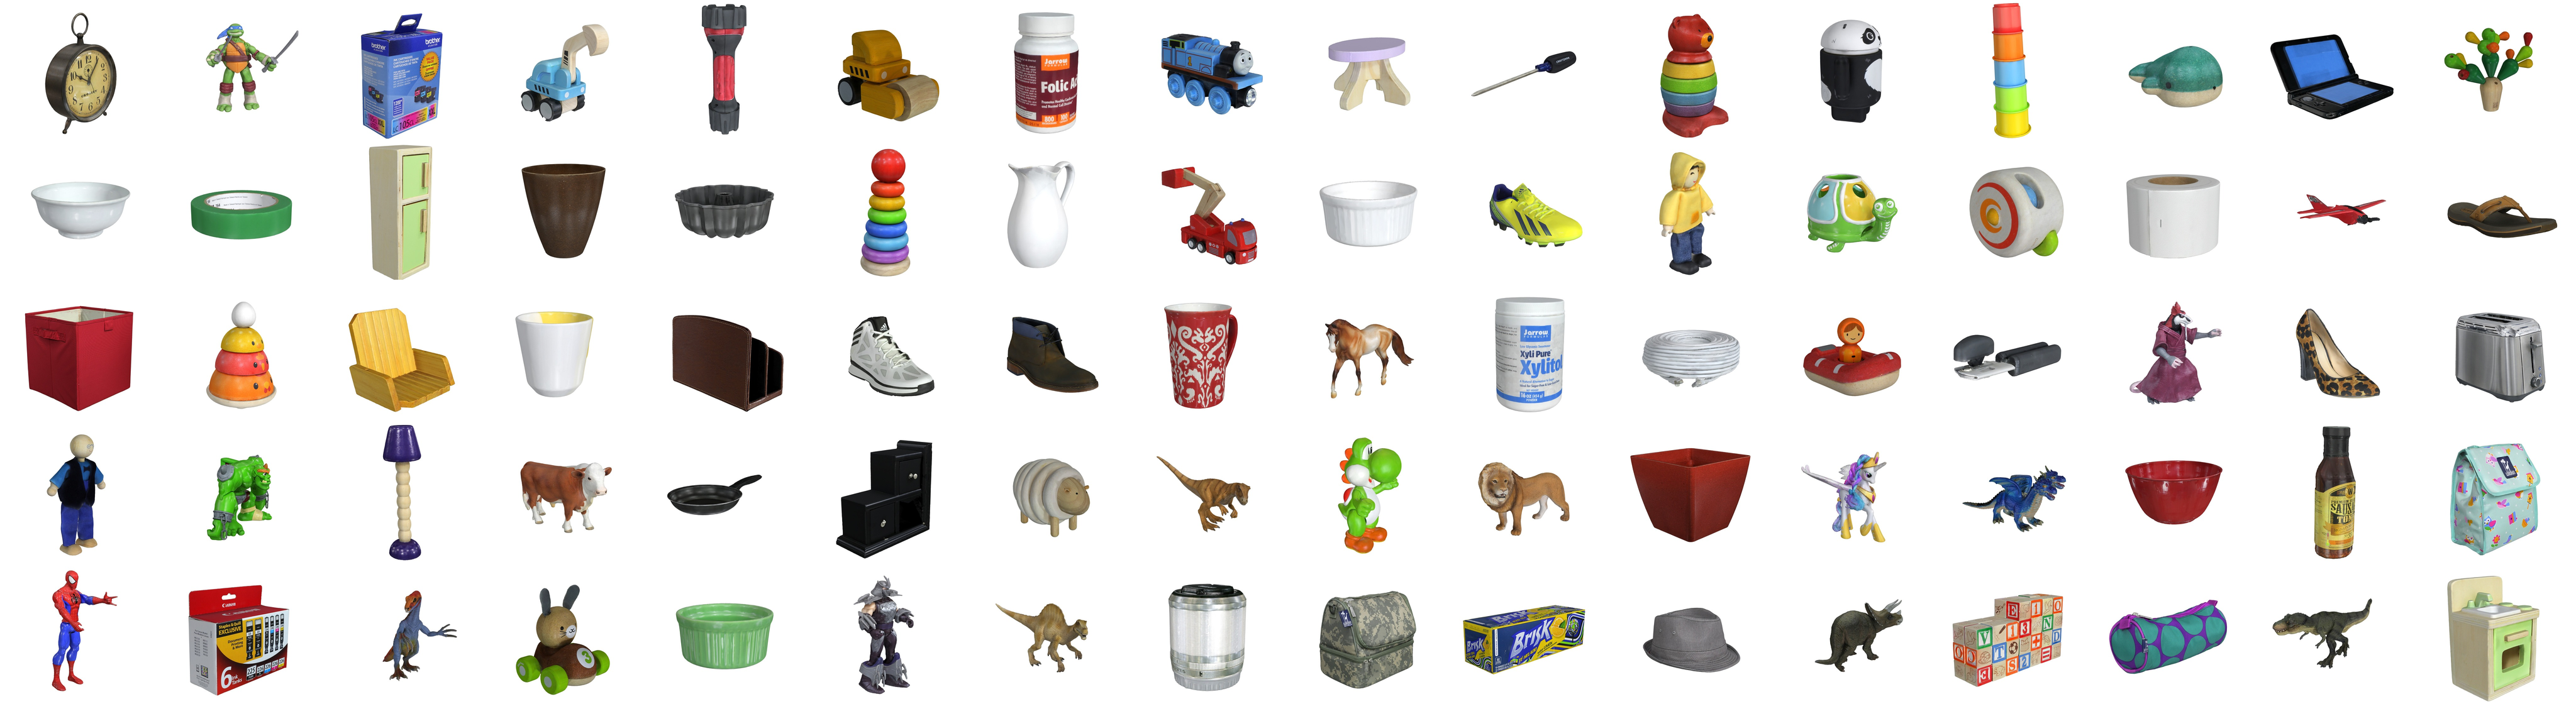
\includegraphics[width=0.995\textwidth]{implementation/training.png}
        \end{flushleft}%
    \end{subfigure}%
    \vrule~%
    \begin{subfigure}[ht]{0.198\textwidth}
        \begin{flushright}%
            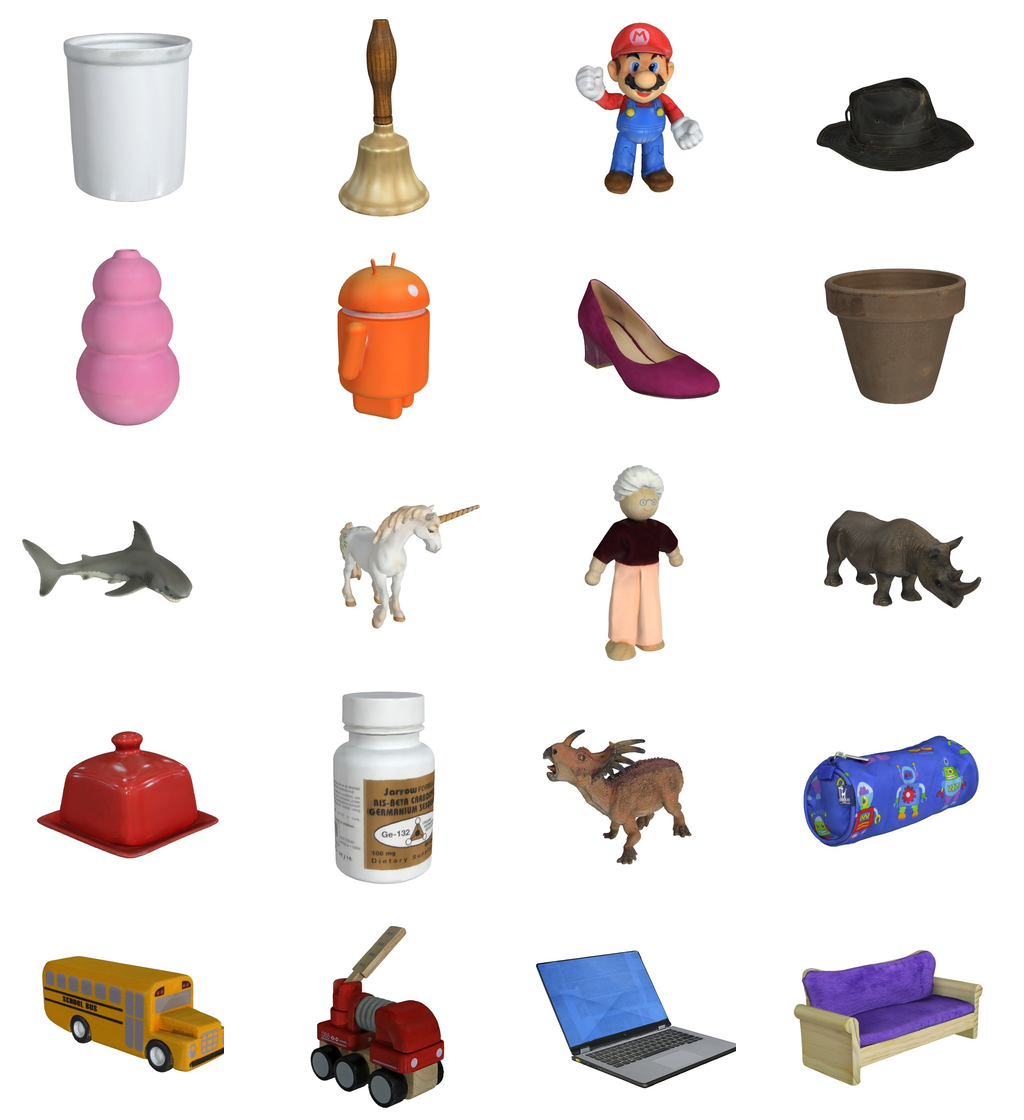
\includegraphics[width=0.995\textwidth]{implementation/testing.png}
        \end{flushright}%
    \end{subfigure}%
    \caption{Training (left) and testing (right) datasets of diverse scanned objects that are utilised in the simulated RL grasping environment. Collection is provided by \citet{googleresearch_google_2020}.}
    \label{fig:dataset}
\end{figure}

All of these objects contain only their corresponding mesh geometry and material texture but lack all other properties. Inertial properties were therefore estimated from their geometry in a procedure that is similar to the aforementioned robot models. Mass of each object used during such estimation was randomly selected alongside other properties of the model, which is detailed below in \autoref{sec:impl_domain_randomisation}. This also include the scale of their geometry, as many of these objects would be too large to fit inside the utilised grippers.

The 3D scanned objects contain meshes with a very high resolution, which makes them unsuitable for computing physical interactions due to the enormous computational cost it would bring. Therefore, a low resolution copy of each mesh is created for use as a collision geometry, alongside the original mesh that is kept for visual appearance. Such copy is automatically generated for each model by simplifying the original mesh geometry though decimation procedure based quadric error metrics by \citet{garland_surface_1997}. The algorithm was configured to reduce the geometry to~2.5\% of the original faces, which was afterward clipped to the range between~[8,~400] faces in order to avoid outliers.


\subsubsection{Performance of Simulation}

Having a performant simulation accelerates the data collection, which can in turn enable faster iteration for RL research due to reduced training duration. Besides reducing computational load by decimating geometry of objects, few more tricks are applied in this work.

\paragraph{Disabling of Collision for Robot Links} During early trials, it was found that a collision never occurs between robot links and the environment. This is primarily because MoveIt~2 is used to plan collision-free trajectories. Furthermore the action space is restricted only to the yaw rotation, which further reduces possible collisions. Therefore, collision geometry of robot links is disabled during the training with aim to bring a slight performance gain. The collision geometry of gripper, i.e.~hand and fingers, is kept enabled for both robots as these are required for interaction with the objects.

\paragraph{Larger Simulation Step Size} As previously mentioned, dynamic properties of robot joints were manually tuned in order to obtain stable manipulation across a variety of control frequencies. The primary purpose of this tuning is to allow the use of larger simulation step size, which determines the rate at which simulation progresses. This in turn affects the accuracy of physics as well as the frequency of low-level controller. A step size of~4~ms is used for the grasping environment because it was found to have a balanced trade-off between physics stability and performance.

\bigskip

With performance in mind, the control rate of RL agent is set to a lower frequency of~2.5~Hz. This is because the agent only provides high-level control, whereas the motion planner and low-level joint controllers take care of interactions that require faster reaction times.
% TODO: Add RTF (test_env)


\subsection{Domain Randomisation}\label{sec:impl_domain_randomisation}

Even though the simulation environment uses objects with realistic appearance and PBR-capable rendering engine, domain randomisation can still provide advantages for sim-to-real transfer as described in \autoref{subsec:sim2real}. Therefore, domain randomisation is applied for several properties at each reset of the environment, i.e.~before the beginning of each episode. Unless otherwise state, uniform distribution is used for sampling of random variables.

\paragraph{Random Objects} At each reset, a number of random objects from the utilised dataset is spawned. Each object is first randomly and uniformly scaled, such that its longest side is between~12.5 and~17.5~cm. Hereafter, object's inertial properties are recomputed to account for the new scale, while also randomising its mass to be in range~[0.05,~0.5]~kg. Lastly~the coefficient of friction for the object is randomised in range~[0.75,~1.5]. In this way, visual, inertial and mechanical properties of each object are random for every episode.

\paragraph{Random Pose of Objects} Besides randomising the type and attributes of each object, the pose at which they spawn is also randomised. It is randomly sampled for each object from a predefined volume in 3D space. In case two objects are overlapping, one of them is spawned again with a new unique pose.

\paragraph{Random Ground Plane Material Textures} To further randomize visuals of the environment at each reset, a random material texture is given to the ground plane on top of which objects are spawned. Similar to the objects,~100 different PBR materials are used with a split of~80/20 for training and testing, respectively. PBR materials are used, therefore, each of them uses four different texture maps, i.e.~albedo, normal, specular and roughness.

\paragraph{Random Camera Pose} In order to further increase variety in observations and provide invariance to camera pose, it is randomised at each reset. The pose of the camera is randomly sampled from an arc around the centre of workspace, except for~\(\pm\)22.5\textdegree\ behind the robot in order to avoid complete occlusion of the scene. Thereafter, a random height for the camera in a range~[0.1, 0.7]~m is selected. The camera is then oriented towards the workspace centre and placed~\(1\)~m away from it. This step is expected to provide significant benefits for sim-to-real transfer by allowing camera to be positioned in a location that is suitable for the real-world setup, instead of trying to reproduce simulation setup as closely as possible.

\paragraph{Random Initial Joint Configuration} Finally, the initial joint configuration of the utilised robot is randomised. At the beginning of each episode, Gaussian noise~\(\mathcal{N}(0, 6\)\textdegree\()\) is added to each joint in the default configuration.

Examples of fully randomised episodes are shown in \autoref{fig:impl_domain_randomisation}. The aim of this variety in observations is to enable sim-to-real transfer that would allow agent to achieve similar degree of success rate in real-world domain after training only in the simulation

\begin{figure}[ht]
    \centering
    % 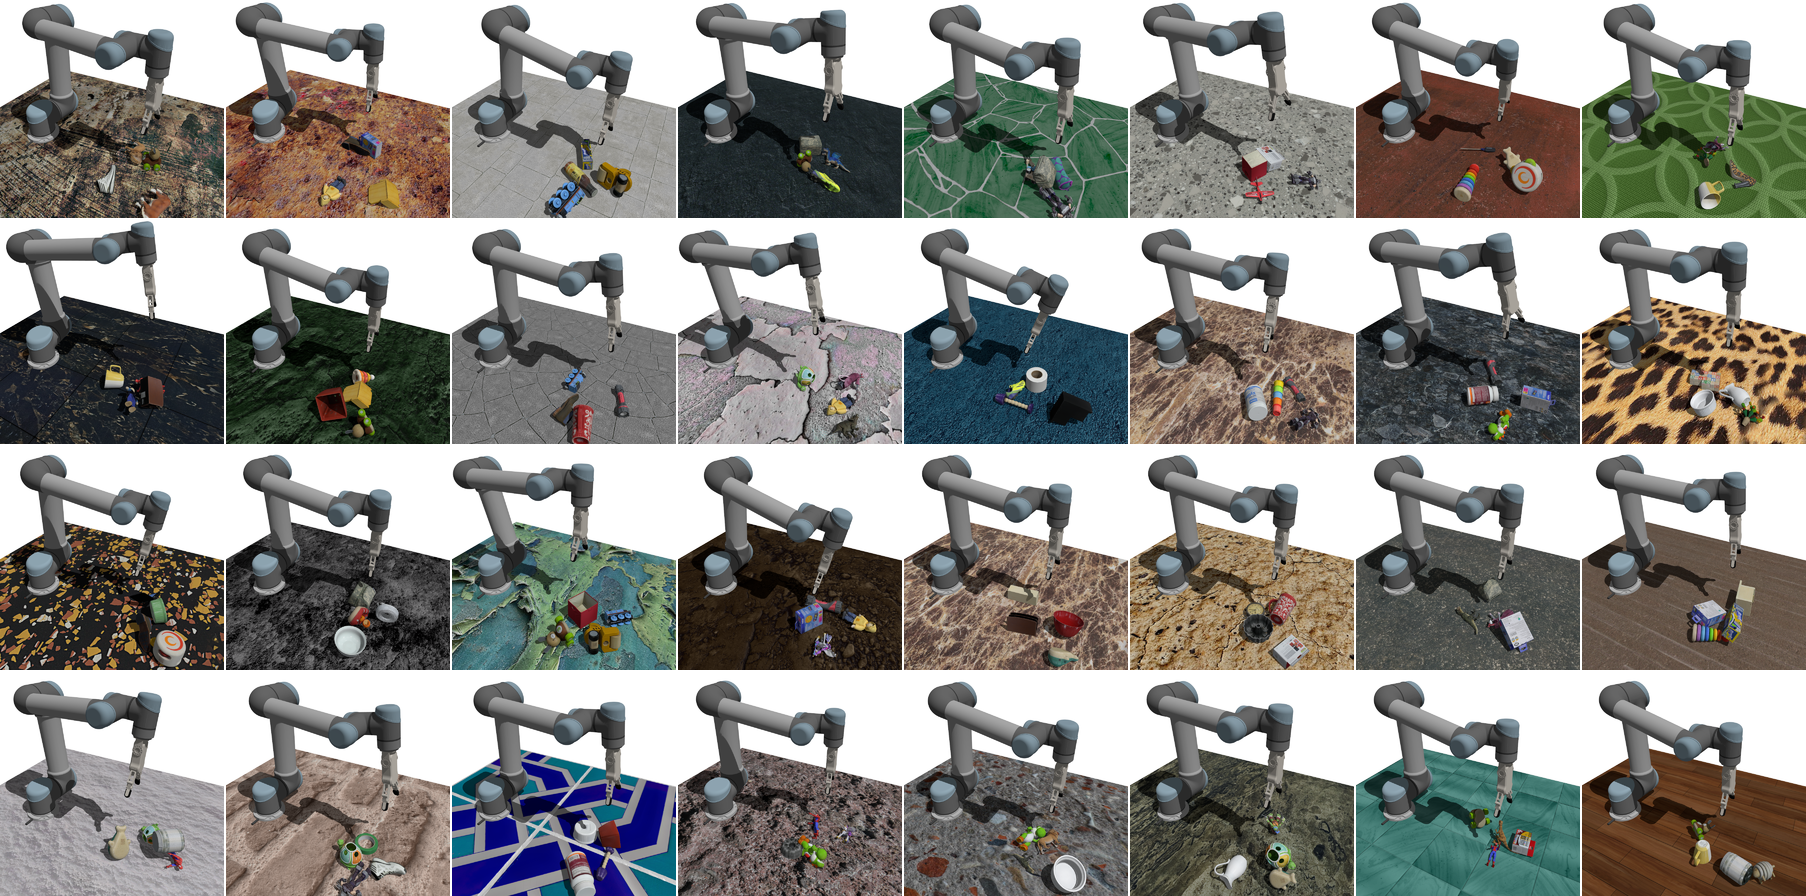
\includegraphics[width=1.0\textwidth]{implementation/domain_randomisation.png}
    \caption{Examples of domain randomisation applied to the implemented simulated environment for robotic grasping.}
    \label{fig:impl_domain_randomisation}
\end{figure}


\subsection{Demonstrations and Curriculum}

As mentioned in \autoref{sec:rw_reinforcement_learning}, demonstrations and curriculum learning can mitigate issues with lengthy exploration. Both of these concepts are therefore investigated in this work and implemented in the following way.

\paragraph{Demonstrations} For demonstrations, approach by \citet{kalashnikov_qt-opt_2018} with the use of a scripted policy is applied. Since off-policy RL algorithms with experience replay buffer are employed, the demonstrations can be simply loaded into such buffer at the beginning of training. More specifically,~\(5000\) transitions are loaded into the replay buffer. The scripted policy is described in \hyperref[app:scripted_policy]{appendix~\ref*{app:scripted_policy}}.

\paragraph{Curriculum} Similar to demonstrations, the use of curriculum can improve learning for tasks in complex environment. This work utilises a curriculum that progressively increases the number of spawned objects and area on top of which these objects are spawned based on current success rate determined by moving average with~\(n\)~=~\(100\). The spawn area increases linearly from~2.4\({\times}\)2.4~cm at~0\% success to~24\({\times}\)24~cm at success rate of~60\%. Similarly, training begins with a single object, with an addition of extra object every~20\% until reaching a maximum of four objects at~60\% success rate.


\section{Deep Reinforcement Learning}

The implementation of DRL in this work focuses on integration of octree-based feature extraction for solving vision-based robotic grasping. A framework for DRL is first selected, which is then followed by description of the architecture of the feature extractor and network for actor and critics. Lastly, the applied process of hyperparameter optimisation is presented.


\subsection{Framework for Reinforcement Learning}

It can be very time-consuming and error-prone to implement DRL algorithms from scratch due to several issues that could arise. Therefore, a framework with pre-existing implementations of the utilised actor-critic algorithms from \autoref{sec:bg_actor_critic_algorithms}, i.e.~TD3, SAC and TQC, is utilised. After a brief investigation of the available frameworks for model-free RL, Stable Baselines3 (SB3) by \citet{raffin_stable-baselines3_2019} was selected due to its reliable implementation of the utilised algorithms, open-source nature and active development. Underneath, SB3 utilises PyTorch \cite{paszke_pytorch_2019} as a machine learning backend that enables training of NNs via its automatic differentiation engine.

In order to enable octree-based feature extraction, the SB3 implementation of algorithms was extended with few modifications. These primarily consisted of support for octrees inside replay buffer, formation of octree batches and integration of the octree-based feature extractor with NNs of actor and critics. All other configuration of the algorithms was performed through their hyperparameters.


\subsection{Feature Extraction}

With visual features, the first part of the network can often be considered as a feature extractor that transforms raw data into more abstract features. This fact is often employed in network architectures for actor-critic DRL methods, where a feature extractor CNN network is shared between the actor and critics. This work therefore utilises the same approach, where a common feature extractor transforms raw input into features that are then provided as input for actor and critic networks. To extract features from octrees, O-CNN implementation by \cite{wang_o-cnn_2017} is used as a base for the employed feature extractor.


\subsubsection{Construction of Octree}

First, an octree is constructed from the aforementioned transformed point cloud of the scene during each step. For this, a volume of~24\({\times}\)24\({\times}\)24~cm is defined to be the observable workspace as a space that is coincidental with the workspace of the robot. Therefore, each point cloud is cropped to occupy only this volume in order to preserve assumption about volumetric 3D data representations from \autoref{subsec:problem_formulation_octree}.

Maximum depth of the octree was selected as~\(d_{max}\)~=~\(4\) in order to provide metric resolution of each finest leaf octant of~1.5\({\times}\)1.5\({\times}\)1.5~cm. This depth was found to provide enough detail for grasping of objects from the utilised dataset, while not slowing down the training due enormous number of cells. Every octree therefore contains a theoretical maximum of~4096 cells, however, an average of~13\% of these cells are occupied at any given time in the created simulation environment. This is primarily because only a single view of the scene is used, where each occlusion prohibits the formation of new cells in the occluded regions behind the visible surfaces. Therefore, it is expected that for each additional depth, the workspace volume can be increased eightfold for the utilised dataset while the actual number of occupied cells would be increased at a much slower rate.

As it was previously described in \autoref{subsec:problem_formulation_octree}, each occupied finest leaf octant contains the average unit normal vector~\(\overline{n}\), the average distance between the centre of the cell and points that formed it~\(\overline{d}\) and the average colour~\(\overline{rgb}\). All of these features are extracted directly from the point cloud that is used to create the octree, where each octet considers only the points that belong to its volume. Since the cropped point cloud does not contain normals, these are estimated for each point from their nearest neighbourhood, where maximum of~10 closest neighbours at a maximum distance of~5~cm are considered. Position of the camera is then used to orient all normals correctly. Once these are found, an octree is created from the point cloud by hierarchical subdivision of the cells. An example of created octree is visualised in \autoref{fig:octree_visualisation}.

\begin{figure}[ht]
    \centering
    % \includegraphics[width=1.0\textwidth]{implementation/octree_visualisation.pdf}
    \caption{Octree that created from a corresponding point cloud of the scene. In this visualisation, each finest leaf octet is represented as a square that is oriented by~\(\overline{n}\) and offset from the centre of the octet by~\(\overline{d}\). Furthermore, each octet is colourised with its corresponding~\(\overline{rgb}\) feature.}
    \label{fig:octree_visualisation}
\end{figure}


\subsubsection{Network Architecture of Feature Extractor}

After octrees are created, NN can use them to extract abstract visual features about the environment. Due to the popularity of CNN architectures for image-based DL, 3D octree-based CNN is employed in this work with. In order to incorporate proprioceptive observations from \autoref{subsec:problem_formulation_proprioceptive_observations}, these are processed only slightly and concatenated with the features extracted from octrees. The developed architecture of the network is represented in \autoref{fig:feature_extractor_architecture}.

\begin{figure}[ht]
    \centering
    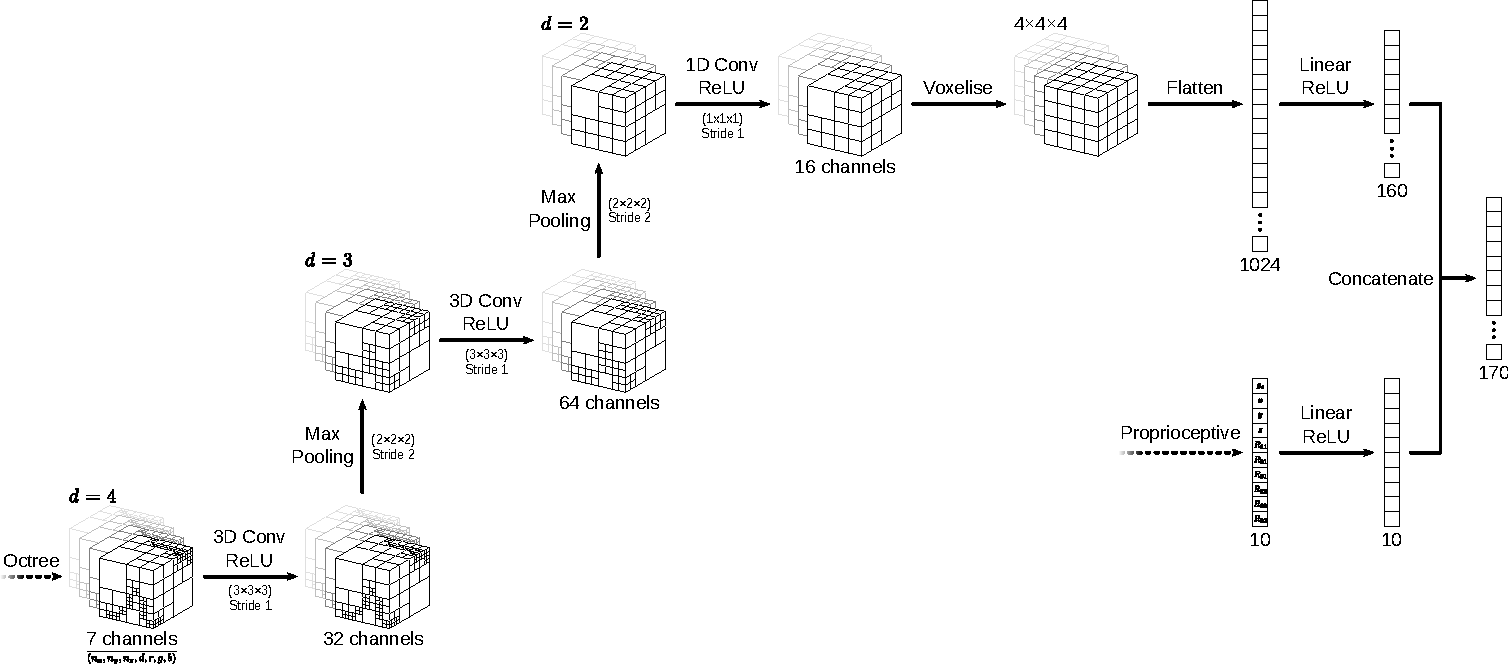
\includegraphics[width=1.0\textwidth]{implementation/feature_extractor.pdf}
    \caption{Architecture of the octree-based CNN feature extractor. Auxiliary features from proprioceptive observations are concatenated to features extracted from octrees in order to provide a single output feature vector. This network is duplicated for each of the three observation stacks and their output is concatenated into a feature vector with length of~510.}
    \label{fig:feature_extractor_architecture}
\end{figure}

The network begins with processing octrees at the maximum depth~\(d\)~=~\(d_{max}\)~=~\(4\). Each octree contains seven channels, which encompass the aforementioned features. From this depth, the octree is processed through a series of 3D convolutions, ReLU (Rectified Linear Unit) activation function and maximum pooling. After each pooling operation, the depth of the octree is decremented such that next convolutional layer computes features that are at a larger scale. This series of modules is applied twice, such that the depth of the octree is reduced to~\(d\)~=~\(2\). While doing so, the dimensionality of channels is increased to provide a wider feature space. However, it is necessary to reduce the number of channels before the next step. For this, 1D convolution is applied in order to compress the feature space by combining together features from the different channels for each cell. Once the dimensionality is reduced, the octree is voxelised in order to acquire a structure that has a static size regardless on the input, which enables use of more traditional DL layers. It is achieved by padding the octree at~\(d\)~=~\(2\) with zeros wherever a cell is not already occupied. Once voxelised, the feature space is flattened into a feature vector that is then processed by a single fully connected layer followed by ReLU activation in order to provide the final set of features from octree observations.

The proprioceptive observations are also processed by the same feature extractor. However, only a single linear layer with ReLU activation and the same dimensionality is used because these features are already at a higher level compared to the raw octrees. Hereafter, the features extracted from octree are combined with proprioceptive features into a single feature vector. The number of utilised channels and the dimensionality of feature vectors is presented in \autoref{fig:feature_extractor_architecture}, which results in total of~226,384 learnable parameters.
% TODO: verify number of parameters, 226590?

In order to enable observation stacking described in \autoref{subsec:observation_stacking}, the feature extractor is duplicated for each of the three stacks. Once all observation stacks are processed individually, their output is concatenated into a single feature vector that can be used by actor and critic networks. A separate network for each stack is utilised instead of a common network because it allows agent to extract different set of features from historical and current observations. The disadvantage of this approach is increased number of parameters that must be learned, which could potentially slow down the training process. Such effect is therefore investigated during experimental evaluation.


\subsection{Actor-Critic Network Architecture}

Once the feature vector is extracted, it can be used as an input for approximator of the utilised algorithm, e.g.~another network or a set of networks. Only actor-critic RL algorithms TD3, SAC and TQC are employed in this work, therefore, a single high-level network architecture can be used for all of them. The implementation of these networks for specific algorithm would differ in the output they provide. For example, SAC and TQC require actor to provide a stochastic policy as opposed to TD3, where TQC also utilises a distributional representation of critic's output.

\autoref{fig:actor_critic_network} illustrates the utilised network architecture that combines a shared feature extractor with actor and critic networks. Identical architecture that consists of two fully connected layers with ReLU activations is employed for both actor and critics, albeit with a separate set of parameters. With the utilised number of nodes, there are~524,288 learnable parameters for each actor and critic network.

\begin{figure}[ht]
    \centering
    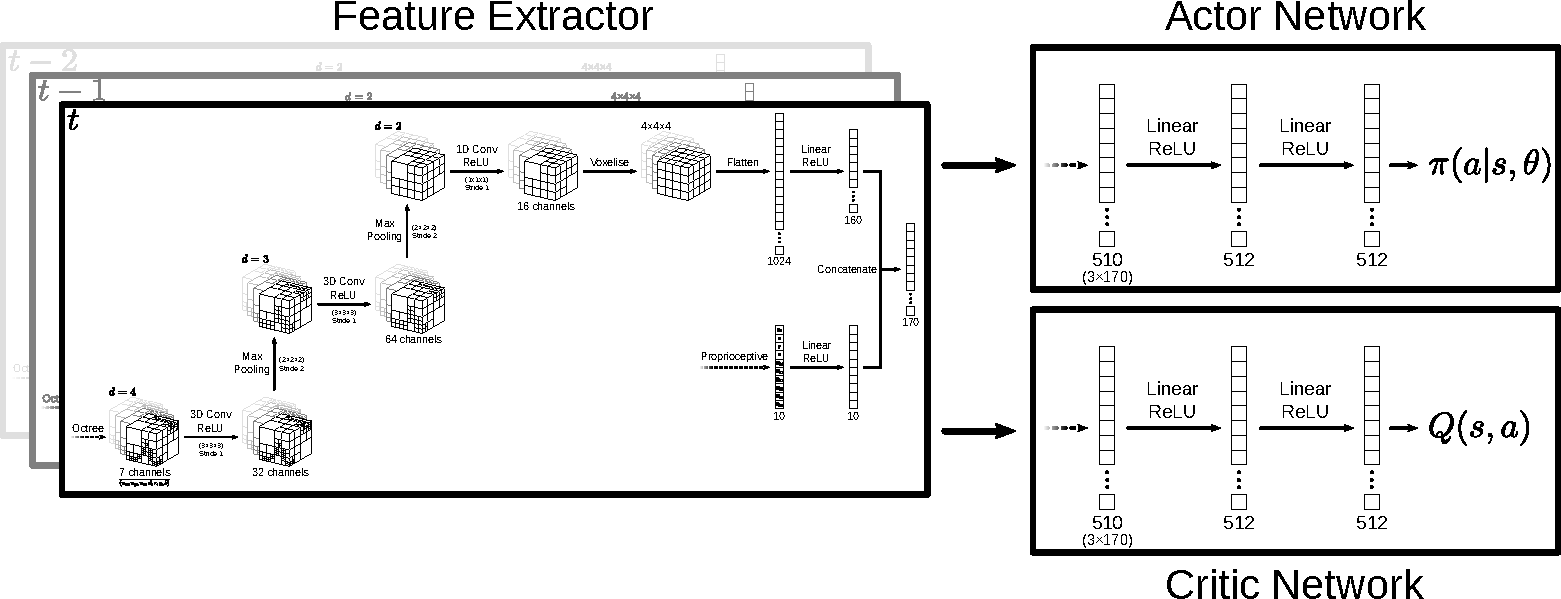
\includegraphics[width=1.0\textwidth]{implementation/actor_critic_network_full.pdf}
    \caption{Network architecture that is used in this work for all utilised actor-critic algorithms. The feature extractor from \protect\autoref{fig:feature_extractor_architecture} is duplicated for each stack in order to process two historical observations in addition to the current one.}
    \label{fig:actor_critic_network}
\end{figure}


\subsection{Hyperparameter Optimisation}

Selection of hyperparameters can significantly affect the learning curve as well as the final performance of a learned policy. This brittleness of DRL to hyperparameters therefore means that their optimisation is of great importance and needs to be performed for each environment. In this work, both automatic optimisation and manual fine-tuning is performed with aim to obtain a set of hyperparameters that would allow robust learning of policy for the created environment, observations and utilised RL algorithms.

First, an automatic hyperparameter optimisation is applied by the use of Optuna, which is a hyperparameter optimisation framework developed by \citet{akiba_optuna_2019}. Optuna and other similar frameworks address the problem of selecting a viable combination of hyperparameters for DL by performing a number of different trials that are used to iteratively search the hyperparameter space and find a combination that provides the best results according to some metric. In terms of RL, this metric is a reward that an agent is able to accumulate over the course of some evaluation period. Optuna generally consists of two parts, which are the sampler and the pruner. Sampler selects a set of hyperparameters from the hyperparameter search-space for the next trial. Such selection can either be completely random, e.g.~at the beginning of an experiment, or by applying algorithms that perform statistical analysis from all previous trials. Pruner in this context is a strategy that allows early stopping of non-promising trials with aim to limit the amount of wasted resources. Pruning requires that evaluation episodes of each trial are run at regular intervals, where each new trial is compared to the performance of all previous trials and pruned if the accumulated reward is comparably too low.

For the grasping environment, Optuna is first applied to optimise hyperparameters in order to get a baseline that provides a reliable performance. This optimisation was performed using SAC, where the search space consisted of most hyperparameters including the size of the feature extractor and actor-critic networks. Size of the replay buffer, batch size and initial entropy were not optimised automatically. Replay buffer and batch size were selected to be adequately large for the utilised system in terms of maximum RAM and VRAM usage, respectively. Initial entropy is kept consistent because it directly influences the performance during the early stages of trials and large initial entropy could result in unwanted pruning of trials. Total of~70 trials with a maximum trial duration of~100,000 time steps were used. A set of~20 evaluation episodes was performed every~25,000 time steps, which could trigger pruning. At the end, the best performing set of hyperparameters was used for subsequent manual tuning.

Manual tuning is applied because the automatic optimisation with Optuna requires a lot of compute time for complex environments such as the one created in this work. This is also the reason why only~70 trials with a maximum trial duration of~100,000 time steps were used, which already took approximately three weeks of compute time. Manual tuning of targetted hyperparameters was therefore performed with several more trials, which were manually initiated and stopped. Focus of this process was mostly on hyperparameters of the implemented environment, e.g.~reward scale, and on the octree-based feature extractor such as the maximum depth and network size. The resulting hyperparameters for all utilised actor-critic algorithms can be seen in \hyperref[app:hyperparameters]{appendix~\ref*{app:hyperparameters}}.
